\documentclass[11pt]{article}
\usepackage[margin=1in]{geometry}
\usepackage{amsmath}
\usepackage{graphicx}
\usepackage{enumitem}
\usepackage{fancyhdr}
\usepackage{tikz}
\usepackage{array}
\usepackage{multirow}
\usepackage{colortbl}

% Header setup
\pagestyle{fancy}
\fancyhf{}
\lhead{Name: \underline{\hspace{3cm}} \quad Period: \underline{\hspace{1cm}}}
\rhead{Date: \underline{\hspace{2.5cm}}}
\cfoot{\thepage}
\renewcommand{\headrulewidth}{0.5pt}

% Custom commands
\newcommand{\blank}[1]{\underline{\hspace{#1}}}

\title{\vspace{-2cm}\textbf{From Candy Auction to Maximum Revenue}\\
\large Finding the Sweet Spot: Price Optimization Through Data}
\author{}
\date{}

\begin{document}
\maketitle
\thispagestyle{fancy}

\section*{Part 1: Reviewing Our Auction Data}

Yesterday, we conducted a candy auction where each group could buy as many candies as they wanted at each price point. Let's organize what we discovered about \textbf{demand} -- how many candies people wanted to buy at different prices.

\subsection*{Step 1: Record Your Auction Results}

Fill in the table below with the data from our 5 auction rounds:

\begin{center}
\renewcommand{\arraystretch}{2}
\begin{tabular}{|c|c|c|}
\hline
\rowcolor{gray!20}
\textbf{Round} & \textbf{Price (\$)} & \textbf{Total Quantity Demanded} \\
& & \textit{(candies bought by all groups)} \\
\hline
1 & \blank{2cm} & \blank{3cm} \\
\hline
2 & \blank{2cm} & \blank{3cm} \\
\hline
3 & \blank{2cm} & \blank{3cm} \\
\hline
4 & \blank{2cm} & \blank{3cm} \\
\hline
5 & \blank{2cm} & \blank{3cm} \\
\hline
\end{tabular}
\end{center}

\subsection*{Step 2: Quick Check on Demand}

\textbf{Question:} Look at your Price vs. Quantity Demanded data. What pattern do you notice?

\vspace{1cm}
\blank{12cm}

\vspace{0.5cm}
\blank{12cm}

This pattern is called the \textbf{Law of Demand} in economics!

\section*{Part 2: From Demand to Revenue}

Now comes the business insight: It's not just about how many we sell -- it's about how much money we make!

\subsection*{Step 3: Calculate Revenue}

For each round, calculate the \textbf{revenue} (total money collected):

\begin{center}
\colorbox{yellow!30}{
\textbf{Revenue = Price $\times$ Quantity Demanded}
}
\end{center}

\vspace{0.5cm}

\begin{center}
\renewcommand{\arraystretch}{2}
\begin{tabular}{|c|c|c|c|}
\hline
\rowcolor{gray!20}
\textbf{Round} & \textbf{Price (\$)} & \textbf{Quantity Demanded} & \textbf{Revenue (\$)} \\
& \textit{(copy from above)} & \textit{(copy from above)} & \textit{(calculate: Price $\times$ Quantity)} \\
\hline
1 & \blank{2cm} & \blank{2cm} & \blank{3cm} \\
\hline
2 & \blank{2cm} & \blank{2cm} & \blank{3cm} \\
\hline
3 & \blank{2cm} & \blank{2cm} & \blank{3cm} \\
\hline
4 & \blank{2cm} & \blank{2cm} & \blank{3cm} \\
\hline
5 & \blank{2cm} & \blank{2cm} & \blank{3cm} \\
\hline
\end{tabular}
\end{center}

\subsection*{Step 4: The Million Dollar Question}

Looking at your revenue column, which price gave you the \textbf{highest revenue}?

Price: \$\blank{2cm} \qquad Revenue at that price: \$\blank{3cm}

\section*{Part 3: Creating the Revenue Graph in Desmos}

\subsection*{Step 5: Plot Price vs. Revenue}

\begin{enumerate}[label=\alph*)]
\item Open Desmos graphing calculator
\item Create a new table with two columns:
    \begin{itemize}
    \item Column 1: Label it $x_1$ (this is Price)
    \item Column 2: Label it $y_1$ (this is Revenue)
    \end{itemize}
\item Enter your 5 data points from the Price and Revenue columns above
\item You should see dots forming a curve!
\end{enumerate}

\textbf{Sketch what you see:}

\begin{center}
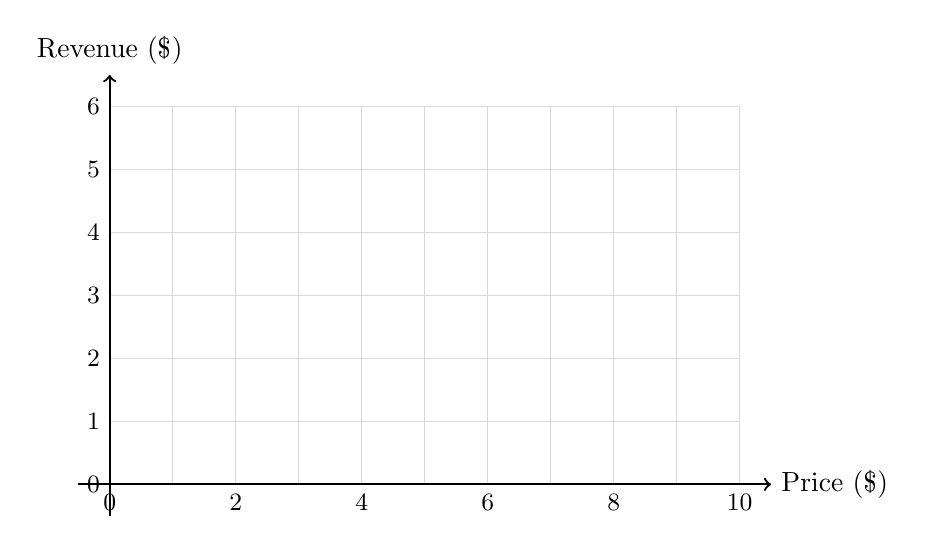
\begin{tikzpicture}[scale=0.8]
% Grid
\draw[gray!30, very thin] (0,0) grid (10,6);
% Axes
\draw[thick, ->] (-0.5,0) -- (10.5,0) node[right] {Price (\$)};
\draw[thick, ->] (0,-0.5) -- (0,6.5) node[above] {Revenue (\$)};
% Add axis labels
\foreach \x in {0,2,4,6,8,10}
    \node[below] at (\x,0) {\small \x};
\foreach \y in {0,1,2,3,4,5,6}
    \node[left] at (0,\y) {\small \y};
\end{tikzpicture}
\end{center}

\section*{Part 4: Finding the Perfect Price with Regression}

\subsection*{Step 6: Fit a Quadratic (Parabola) to Your Data}

In Desmos, type this in a new line:
\begin{center}
\colorbox{blue!10}{\texttt{$y_1 \sim ax_1^2 + bx_1 + c$}}
\end{center}

Desmos will automatically find the best-fitting parabola! Write the equation it gives you:

\vspace{0.5cm}
\begin{center}
\fbox{
$R(p) = \blank{2cm} \, p^2 + \blank{2cm} \, p + \blank{2cm}$
}
\end{center}

Record the values Desmos calculated:
\begin{itemize}
\item $a = $ \blank{3cm} (this should be negative because our parabola opens down and has a maximum)
\item $b = $ \blank{3cm}
\item $c = $ \blank{3cm}
\end{itemize}

\section*{Part 5: The Vertex -- Your Optimal Price!}

The highest point on your revenue parabola is called the \textbf{vertex}. This tells you the best price to charge!

\subsection*{Step 7: Find the Vertex Graphically}

\begin{enumerate}[label=\alph*)]
\item Click on the highest point of your parabola in Desmos
\item Desmos will show you the coordinates: (Price, Revenue)
\end{enumerate}

\textbf{Vertex from Graph:} \quad Price = \$\blank{2cm} \quad Maximum Revenue = \$\blank{3cm}

\subsection*{Step 8: Find the Vertex Using Algebra}

For any parabola $y = ax^2 + bx + c$, the x-coordinate of the vertex is:

\begin{center}
\colorbox{yellow!30}{
$x = -\dfrac{b}{2a}$
}
\end{center}

Using your values of $a$ and $b$ from Step 6:

\vspace{0.5cm}
\begin{align*}
\text{Optimal Price} &= -\dfrac{b}{2a}\\[0.5cm]
&= -\dfrac{\blank{3cm}}{2 \times (\blank{3cm})}\\[0.5cm]
&= -\dfrac{\blank{3cm}}{\blank{3cm}}\\[0.5cm]
&= \$\blank{3cm}
\end{align*}

\textbf{Check:} Does this match what you found graphically? \quad Yes \quad No

\section*{Part 6: Making Business Sense}

\subsection*{Step 9: Interpret Your Results}

Complete these sentences based on your analysis:

\begin{enumerate}[label=\alph*)]
\item If we price the candy too low (like \$\blank{1.5cm}), we sell a lot but don't make much per candy,
so our total revenue is \blank{5cm}.

\item If we price the candy too high (like \$\blank{1.5cm}), we make a lot per candy but \blank{5cm},
so our total revenue is also low.

\item The ``sweet spot'' price that maximizes our revenue is \$\blank{1.5cm},
which would give us a revenue of \$\blank{2cm}.
\end{enumerate}

\subsection*{Step 10: Business Recommendation}

Write a 2-3 sentence recommendation to a candy store owner based on your analysis:

\vspace{1cm}
\hrule
\vspace{1cm}
\hrule
\vspace{1cm}
\hrule
\vspace{1cm}
\hrule

\section*{Extension Question (if time allows)}

\textbf{Think About It:} We found the price that maximizes \textit{revenue}, but businesses care about \textit{profit}.
What additional information would we need to find the price that maximizes profit instead?

\vspace{1cm}
\blank{12cm}

\vspace{0.5cm}
\blank{12cm}

\vspace{2cm}

\begin{center}
\rule{0.8\textwidth}{0.5pt}

\textit{Next Class: We'll apply these same techniques to help real local businesses (Golden Monkey, Mandee's, and Yas Chicken) find their optimal prices!}
\end{center}

\end{document}